Avant toute chose, créer un répertoire \lstinline{TP08} dans votre répertoire \lstinline{Informatique}, \lstinline{TPsup} dans votre espace personnel.

Sur le site \url{https://ptsilamartin.github.io/info/TP.html}, télécharger les 2  images \href{https://ptsilamartin.github.io/info/TP/allium.png}{allium.png}
\lstinline{allium.png}, \href{https://ptsilamartin.github.io/info/TP/ciel.png}{ciel.png} ainsi que le script \href{https://ptsilamartin.github.io/info/TP/TP_08.py}{TP\_08.py}  que vous copiez dans votre répertoire TP08. Ouvrir le script \lstinline{TP08.py} dans lequel vous travaillerez tout au long de ce TP.

\section*{Créer des images en niveau de gris}



\begin{marginfigure}
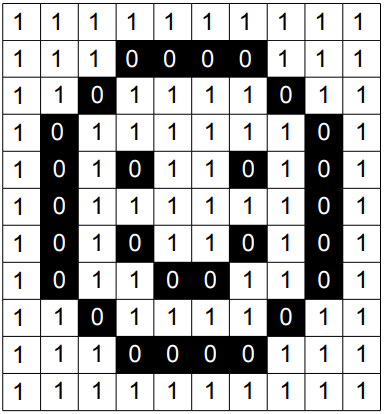
\includegraphics[width=\textwidth]{codage1.png}
\end{marginfigure}
Dans ce TP nous utilisons sur des \textbf{images matricielles} (formées de points, les pixels). 

Le codage d'une image se fait alors sous la forme d'une matrice. Chaque pixel de l'image correspond à un élément de la matrice.

Ci-contre une image ne contenant que du noir (codé par un 0) et du blanc (codé par un 1).


Les images dites en "noir et blanc" sont en fait des images en dégradé de gris (ou niveaux de gris). Chaque élément de la matrice correspondra comme précédemment à un pixel, mais ces éléments seront des flottants (compris entre 0. et 1.) donnant l'intensité de gris voulue. On utilise ici le 0 pour le noir et le 1 pour le blanc. Une valeur de 0.5 sera un gris moyen, de 0.2 un gris foncé et de 0.8 un gris clair.

\begin{question}
Compléter les commentaires de la fonction \lstinline{image_noire} fournie dans le script \lstinline{TP08.py}. Appeler ensuite cette fonction pour créer une image noire de largeur 6 pixels et de hauteur 3 pixels.
\end{question}

\begin{question}
Afficher la matrice obtenue dans le script. Afficher ensuite  l'image obtenue dans une figure \lstinline{matplotlib} comme indiqué ci-dessous.
\end{question}

\begin{lstlisting}
import matplotlib.pyplot as plt  # importation de la bibliothèque matplotlib

plt.figure("NOM de la figure")  # crée une nouvelle figure
plt.imshow(im,cmap='gray',vmin=0, vmax=1)  # affiche l'image codée par la matrice im  /en niveau de gris, les pixels étant codés par des valeurs allant du 0 au 1 
\end{lstlisting}


\begin{question}
\'Ecrire les fonctions \lstinline{rayure_hor} et \lstinline{rayure_ver} qui créent des images rayées horizontalement et verticalement. Tester ces fonctions sur des images de hauteur 9 et de largeur 14. Afficher les résultats obtenus.
\end{question}


\begin{question}
\textbf{BIS (OPTIONNELLE : si vous êtes en avance uniquement)} \'Ecrire la fonction \lstinline{echiquier} qui crée une image avec un motif d'échiquier. Tester et afficher l'image obtenue.
\end{question}


\section*{Eclaircir une image}
Dans cette partie on souhaite éclaircir l'ensemble d'une image.

\begin{question}
\'Ecrire la fonction \lstinline{eclaicir} qui prend pour argument la matrice-image \lstinline{im} et le flottant \lstinline{k} et qui modifie chaque pixel de l'image pour éclaircir d'une valeur \lstinline{k} chaque pixel. (plus la valeur de \lstinline{k} sera élevée plus l'éclaircissement sera conséquent).

Tester ensuite votre fonction sur l'image rayée horizontalement que vous avez obtenue précédemment. Les bandes noires doivent devenir grises. 

Afficher 3 figures : l'image rayée initiale, l'image rayée éclaicie et l'image rayée initiale après application de la fonction \lstinline{eclaicir}.  
\end{question}


\textit{Si on ne prend pas de précautions particulières, le fait d'apliquer la fonction \lstinline{eclaicir} modifie l'image source. Ceci peut être génant si ce n'est pas volontaire. Il faut bien veiller à créer une \textbf{copie indépendante} de la matrice-image source pour éviter ce problème.}

\textbf{Copie indépendante}

\begin{question}
Réécrire la fonction \lstinline{eclaicir2} en ajoutant les commandes permettant de réaliser une copie indépendante de la matrice-image source avant de la modifier. Tester en affichant les 3 figures de la question précédente.
\end{question}


\textbf{Lecture d'une image contenue dans un fichier .png}
On va maintenant appliquer cette fonction sur une autre image, contenue dans le fichier \textbf{allium.png}.

Pour lire un fichier et obtenir la matrice-image correspondante on utilise l'instruction :
\begin{lstlisting}
import matplotlib.image as img   # import d'une autre bibliothèque de matplotlib
imF = img.imread("nom_du_fichier.png")  # lecture du fichier
\end{lstlisting}

\marginnote{\textbf{Attention :} Il faut que le fichier lu se situe dans le même répertoire que le script. Veillez donc à ce que vos fichiers \lstinline{allium.png} et \lstinline{TP08.py} soient dans le même répertoire. Il faudra ensuite exécuter le script en effectuant un clic droit sur l'onglet de votre script puis \textbf{Exécuter en tant que script}.}

 
\begin{question}
Lire le fichier \textbf{allium.png} et stocker la matrice image obtenue dans la variable \textbf{imF}. Afficher cette image. Eclaircir l'image d'une valeur de 0.2 par exemple. Observer l'image obtenue. Vérifier que la matrice-image source \textbf{imF} n'est pas modifée. 
\end{question}



\section*{Détecter les contours}

\textit{La reconnaissance de formes dans une image est une composante importante de l'analyse d'images.
Elle se décompose en plusieurs étapes qui consistent à extraire les contours des objets dans l'image afin
de les reconnaitre ou d'en détecter le mouvement. La première de ces étapes est la mise en évidence
des contours des objets dans l'image. C'est cette étape que nous allons aborder très succinctement.}
\\

\begin{figure}[!h]
\centering
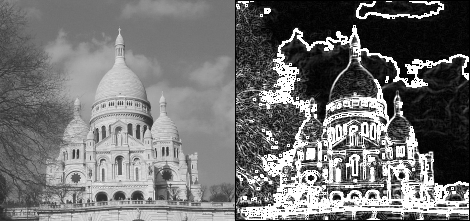
\includegraphics[width=1\textwidth]{edges.png}
\end{figure}

Un contour définit la limite d'un objet dans une image. Cette limite est caractérisée par un changement
dans l'image : un changement de couleur ou de contraste. Ce changement se traduit dans la valeur des pixels qui sont localisés de part et d’autre de la limite.
Nous sommes donc à la recherche d’un moyen de détecter et de localiser un changement.\\

\begin{marginfigure}
\centering
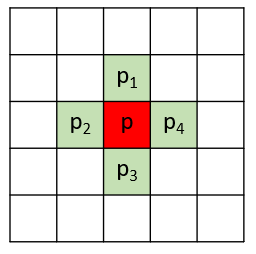
\includegraphics[width=.8\textwidth]{imagepixels.png}
\end{marginfigure}


Considérons un pixel \textbf{p} dans une image. Ce pixel est-il semblable, de même teinte, que ses voisins ? Si non, quelle est la différence de teinte entre lui et ses voisins ? Est-elle grande, ce qui signifierait qu’il est situé à la limite d’un objet ?\\
Le principe est pour chaque pixel de l'image, de récupérer la valeur de chaque pixel avoisinant ce pixel, puis de mesurer la différence, la ”distance” euclidienne, entre ces valeurs en utilisant une fonction de norme standard :
$$
\text{distance}=\sqrt{(p_1-p_3)^2+(p_2-p_4)^2}.
$$



 où $ p_1$, $p_2$, $ p_3$ et $ p_4$ sont les valeurs des 4 pixels voisins.


Après avoir calculé la distance entre les valeurs des voisins du pixel courant, on compare cette distance à une valeur seuil :
\begin{itemize}
\item si la distance est plus petite ou égale que le seuil : la variation est faible : ce pixel n'est pas considéré sur un contour : on le laisse en noir ;
\item si la distance est plus grande strictement que le seuil : la variation est grande : ce pixel est sur le contour : on le trace en blanc.
\end{itemize}


\begin{question}
Lire l'image \lstinline{ciel.png}. Afficher cette image dans une nouvelle figure en utilisant le module \lstinline{matplotlib.pyplot}.
\end{question}



\begin{question}
\'Ecrire une fonction \lstinline{contour}, qui prend comme argument une image en niveaux de gris \lstinline{im} ainsi qu'un flottant \lstinline{seuil}, et qui renvoie une image noire sauf les pixels situés sur le contour qui seront en blanc.
\end{question}

\begin{question}
Tester cette fonction sur l'image  \lstinline{ciel.png}, avec un seuil de 0.2.
\end{question}

